\documentclass[t,24pt]{beamer}

\usepackage[english]{isodate}
\usepackage{KUstyle}
\usepackage{multicol}
\usepackage{amsthm}
\usepackage{amsfonts}
\usepackage{amsmath}
\usepackage{amssymb}
\usepackage[normalem]{ulem}
\usepackage{tikz}
\usepackage{xcolor}
\usepackage{centernot}
\usepackage[T1]{fontenc}
\usepackage{lmodern}

\makeatletter
% Load the OT1 definitions for lmodern
\input{ot1lmr.fd}
% Change the definition for \OT1/lmr/m/n/<size>
\DeclareFontShape{OT1}{lmr}{m}{n}%
  {<-5.5>    rm-lmr5  <5.5-6.5> rm-lmr6
   <6.5-7.5> rm-lmr7  <7.5-8.5> rm-lmr8
   <8.5-9.5> rm-lmr9  <9.5->    rm-lmr10
  }{}

\renewcommand{\arraystretch}{1.25}
\toplinje{Parallel LL Parsing}

\begin{document}

{
\setbeamertemplate{background}{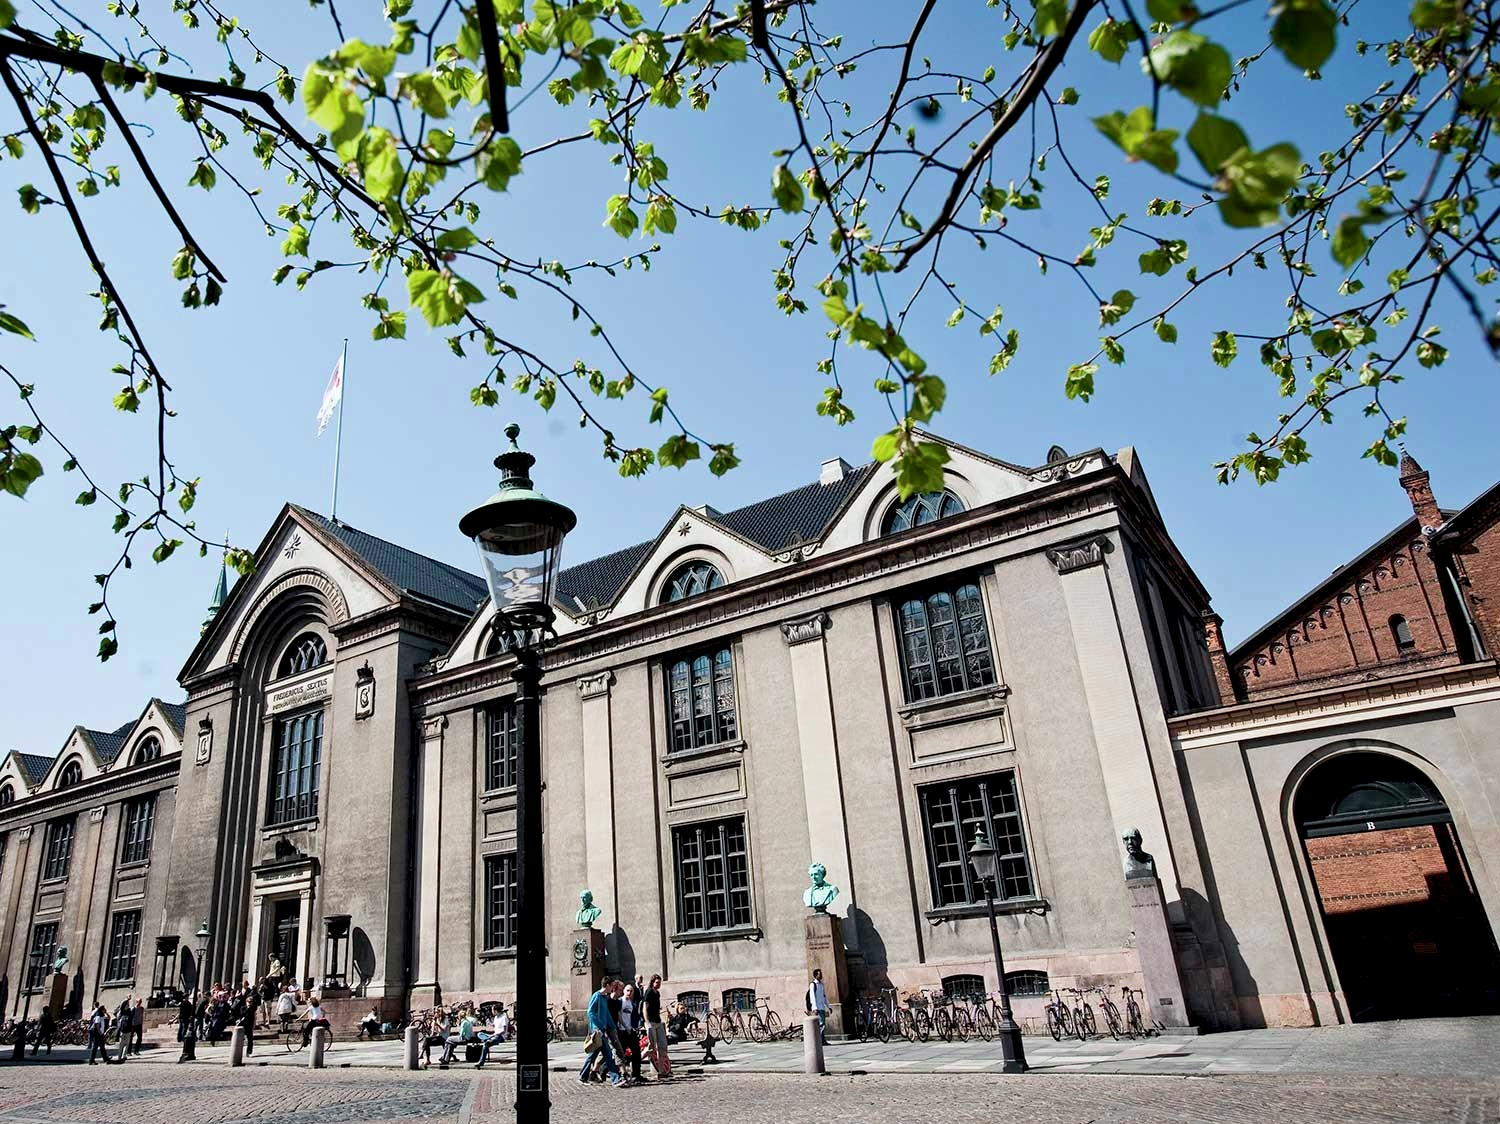
\includegraphics[width=\paperwidth,height=\paperheight]{images/frontpage.jpg}}
\begin{frame}
    \begin{textblock*}{\textwidth}(0.57\textwidth,0.1\textheight)
        \begin{beamercolorbox}[wd=6.4cm,ht=7.7cm,sep=0.5cm]{hvidbox}
            \fontsize{4}{10}\fontfamily{ptm}\selectfont \textls[200]{KØBENHAVNS UNIVERSITET}
            \noindent\textcolor{KUrod}{\rule{5.4cm}{0.4pt}}
        \end{beamercolorbox}
    \end{textblock*}
    \begin{textblock*}{\textwidth}(0.57\textwidth,0.1\textheight)
        \begin{beamercolorbox}[wd=6.4cm,sep=0.5cm]{hvidbox}
            \Huge \textcolor{KUrod}{Parallel Parsing}
            \vspace{0.5cm}
            \par
            \Large The Implementation of a Parallel LL Parser Generator
            \vspace{0.5cm}
            \par
            \normalsize William Henrich Due
            \vspace{0.1cm}
            \par
            30th June 2023
        \end{beamercolorbox}
    \end{textblock*}
    \begin{textblock}{1}(14.2,11.44)
        
\includegraphics[width=1cm]{KU/KU-logo.png}
    \end{textblock}
\end{frame}
}

\begin{frame}[hvid]
    \frametitle{Introduction}
    \begin{itemize}
        \item Parallel LL parser generator.
        \item LLP$(q,k)$ $\subseteq$ LL$(k)$.
        \item Pareas uses LLP$(1, 1)$.
        \item Two mistakes in the paper that describes LLP.
        \item Tested the parser generator thoroughly.
    \end{itemize}
\end{frame}

% \begin{frame}[hvid]
%     \frametitle{What will I be talking about.}
%     \begin{itemize}
%         \item How LLP parsing work.
%         \item One of the problems found.
%         \item Mistakes I made.
%         \item The usefulness of the parser generator.
%         \item A small example showing the parser generator being used.
%     \end{itemize}
% \end{frame}

\begin{frame}[hvid,noframenumbering]
    \frametitle{LL parsing}
    Here is a LL(1) grammar.
    \begin{align*}
        1)\:\: T \to R \qquad 2)\:\: T \to aTc \qquad 3)\:\: R \to \varepsilon \qquad 4)\:\: R \to bR
    \end{align*}
    \begin{align*}
        \onslide<2->{(abc, T, ())} & \onslide<3->{\vdash (abc, aTc, 2)} \onslide<4->{\vdash (bc, Tc, 2)} \onslide<5->{\vdash (bc, Rc, (2, 1))} \\
                                   & \onslide<6->{\vdash (bc, bRc, (2, 1, 4))} \onslide<7->{\vdash (c, Rc, (2, 1, 4))}                         \\
                                   & \onslide<8->{\vdash (c, c, (2, 1, 4, 3))} \onslide<9->{\vdash (\varepsilon, \varepsilon, (2, 1, 4, 3))}
    \end{align*}
    \onslide<9->{Accepted! the string ``$abc$'' can be parsed.}
\end{frame}

\begin{frame}[hvid]
    \frametitle{LLP Parsing}
    Augment the grammar, this grammar is LL(1) and LLP(1, 1).
    \begin{align*}
        0)\:\: T' \to \:\: \vdash T \dashv
    \end{align*}
    Now we parse the string ``$\vdash abc \dashv$'' instead and a LLP table is needed.
    \begin{enumerate}
        \item Initial pushdown store.
        \item Final pushdown store.
        \item Left parse.
    \end{enumerate}
    \only<1>{{\footnotesize
        \begin{center}
            \begin{tabular}{c|c|c|c|c|c}
                                & $\vdash$           & $a$        & $b$           & $c$                      & $\dashv$                      \\ \hline
                $\varepsilon$ & $(T', T\dashv, 0)$ &            &               &                          &                               \\ \hline
                $\vdash$      &                    & $(T,Tc,2)$ & $(T,R,(1,4))$ &                          & $(T\dashv,\varepsilon,(1,3))$ \\ \hline
                $a$           &                    & $(T,Tc,2)$ & $(T,R,(1,4))$ & $(Tc,\varepsilon,(1,3))$ &                               \\ \hline
                $b$           &                    &            & $(R,R, 4)$    & $(Rc,\varepsilon,3)$     & $(R\dashv,\varepsilon,3)$     \\ \hline
                $c$           &                    &            &               & $(c,\varepsilon,())$     & $(\dashv,\varepsilon,())$
            \end{tabular}
        \end{center}
    }}
    \only<2>{
        \begin{center}
            \begin{tabular}{c|c|c|c|c}
                (\varepsilon ,\vdash) & $(\vdash, a)$ & $(a, b)$        & $(b, c)$             & $(c, \dashv)$               \\ \hline
                $(T',T\dashv,0)$      & $(T, Tc, 2)$  & $(T, R, (1,4))$ & $(Rc,\varepsilon,3)$ & $(\dashv, \varepsilon, ())$
            \end{tabular}
        \end{center}
    }
\end{frame}

\begin{frame}[hvid]
    \frametitle{LLP Parsing using Parallel Reduce}
    Use the \uline{associative} $\mathbf{glue}$ operation.
    \vfill
    \begin{center}
        \begin{tikzpicture}[
                level distance=1cm,
                level 1/.style={sibling distance=3cm},
                level 2/.style={sibling distance=4cm},
                level 3/.style={sibling distance=2cm}]
            \node {$({\only<5>{\color{orange}} T'}, {\only<5>{\color{blue}} \varepsilon}, {\only<6>{\color{red}} (0, 2, 1, 4, 3)})$}
            child {node {$({\only<5>{\color{orange}} \only<4>{\color{orange}} T'}, {\only<4>{\color{green}} \only<5>{\color{red}} \dashv}, (0, 2, 1, 4, 3))$}
                    child {node {$({\only<4>{\color{orange}} \only<2>{\color{orange}} T'}, {\only<4>{\color{red}} \only<2>{\color{blue}} Tc}{\only<4>{\color{green}} \only<2>{\color{green}}\dashv}, (0, 2))$}
                            child {node {$({\only<2>{\color{orange}} T'}, {\only<2>{\color{red}} T} {\only<2>{\color{green}} \dashv},0)$}}
                            child {node {$({\only<2>{\color{red}} T}, {\only<2>{\color{blue}} Tc}, 2)$}}
                        }
                    child {node {$({\only<4>{\color{red}} \only<3>{\color{blue}} T} {\only<4>{\color{red}} \only<3>{\color{green}} c}, {\only<4>{\color{blue}} \only<3>{\color{orange}} \varepsilon}, (1,4,3 ))$}
                            child {node {$({\only<3>{\color{blue}} T}, {\only<3>{\color{red}} R}, (1,4))$}}
                            child {node {$({\only<3>{\color{red}} R}{\only<3>{\color{green}} c}, {\only<3>{\color{orange}} \varepsilon},3)$}}
                        }}
            child {node {$({\only<5>{\color{red}} \dashv}, {\only<5>{\color{blue}} \varepsilon}, ())$}};
        \end{tikzpicture}
    \end{center}
    \vfill
\end{frame}

\begin{frame}[hvid]
    \frametitle{LLP Parsing using Bracket Matching}
    \begin{center}
        \begin{tabular}{c|c|c|c|c}
            (\varepsilon ,\vdash)          & $(\vdash, a)$   & $(a, b)$        & $(b, c)$               & $(c, \dashv)$                             \\ \hline
            $(T',T\dashv,0)$               & $(T, Tc, 2)$    & $(T, R, (1,4))$ & $(Rc,\varepsilon,3)$   & $(\dashv, \varepsilon, ())$ \onslide<2->{ \\ \hline
            $(T',T\dashv)$                 & $(T, Tc)$       & $(T, R)$        & $(Rc,\varepsilon)$     & $(\dashv, \varepsilon)$} \onslide<3->{    \\ \hline
            $(T',\dashv T)$                & $(T, cT)$       & $(T, R)$        & $(Rc,\varepsilon)$     & $(\dashv, \varepsilon)$}   \onslide<4->{  \\ \hline
            $(\varepsilon, [^\dashv [^T )$ & $(]^T, [^c[^T)$ & $(]^T, [^R)$    & $(]^R]^c,\varepsilon)$ & $(]^\dashv, \varepsilon)$}
        \end{tabular}
    \end{center}
    \onslide<5->{Now perform bracket matching and assert their types match up.
        \begin{align*}
            {\color{brown} [^\dashv} {\color{blue} [^T ]^T} {\color{green} [^c}{\color{orange} [^T ]^T} {\color{purple} [^R ]^R} {\color{green} ]^c} {\color{brown} ]^\dashv}
        \end{align*}}
    \onslide<6->{
        Construct the production sequence.
        \begin{align*}
            0, 2, 1, 4, 3
        \end{align*}
    }
\end{frame}

\begin{frame}[hvid]
    \frametitle{Syntax Tree}
    \begin{gather*}
        1)\:\: E \to TE' \quad 2)\:\: E' \to +TE' \quad 3)\:\: E' \to \varepsilon \quad 4)\:\: T \to a \\[7pt]
        (a+[a + a], E, ()) \vdash^* (\varepsilon, \varepsilon, (1, 4, 2, 5, 1, 4, 2, 4, 3, 3))
    \end{gather*}
    \begin{center}
        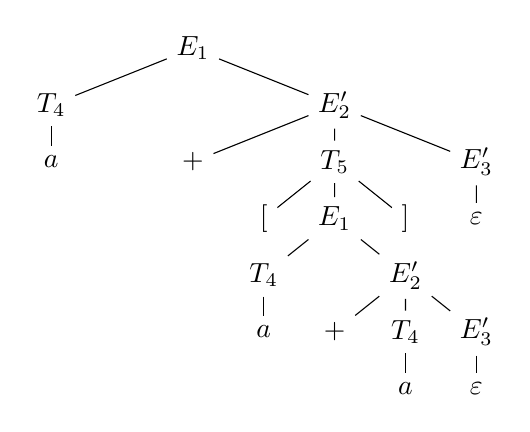
\begin{tikzpicture}[
                scale=0.90,
                level distance=0.8cm,
                level 1/.style={sibling distance=4cm},
                level 2/.style={sibling distance=2cm},
                level 3/.style={sibling distance=1cm},
                level 4/.style={sibling distance=2cm},
                level 5/.style={sibling distance=1cm}]
            \node {$E_1$}
                child {node {$T_4$}
                    child {node {$a$}}
                }
                child {node {$E'_2$}
                    child {node {$+$}}
                    child {node {$T_5$}
                        child {node {$[$}}
                        child {node {$E_1$}
                            child {node {$T_4$}
                                child {node {$a$}}
                            }
                            child {node {$E'_2$}
                                child {node {$+$}}
                                child {node {$T_4$}
                                child {node {$a$}}
                                }    
                                child {node {$E'_3$}
                                    child {node {$\varepsilon$}}  
                                }
                            }
                        }
                        child {node {$]$}}
                    }
                    child {node {$E'_3$}
                        child {node {$\varepsilon$}}  
                    }
                };
        \end{tikzpicture}
    \end{center}
\end{frame}

\begin{frame}[hvid]
    \frametitle{LLP Table}
    To perform LLP parsing a LLP table is needed.
    \begin{enumerate}
        \item Find the initial pushdown.
        \item Parse the first symbol of the lookahead string to get the final pushdown store.
        \item Construct LLP configuration.
    \end{enumerate}
\end{frame}


\begin{frame}[hvid]
    \frametitle{The Problem}
    Consider the following augmented $\text{LL}(2)$ grammar.
    \begin{align*}
        0)\:\: S' \to \: \vdash S \dashv \qquad 1)\:\: A \to \varepsilon \qquad 2)\:\: S \to aAa \qquad 3)\:\: A \to a
    \end{align*}
    \onslide<2->{The PSLS (Prefix of a Suffix of a Leftmost Sentential) table. The grammar is LLP(2,2) since all the sets are singletons.
    {\small
    \begin{center}
        \begin{tabular}{c|c|c|c}
                        & $\dashv$     & $a\dashv$ & $aa$    \\ \hline
            $\vdash$   &              &           & $\{S\}$ \\\hline
            $\vdash a$ &              & $\{A\}$   & $\{A\}$ \\\hline
            $aa$       & $\{\dashv\}$ & $\{a\}$   &
        \end{tabular}
    \end{center}
    }
    }
    \onslide<3->{
        A small example of a PSLS value.
        \begin{align*}
            S \Rightarrow^*_{lm} \:\: \vdash S \dashv \:\: \Rightarrow \:\: \vdash a A a \dashv \:\: \Rightarrow^* \:\: \vdash a a \dashv
        \end{align*}
        This corresponds to the entry $\text{PSLS}(\vdash a, a \dashv) = \{A\}$.
    }
\end{frame}

\begin{frame}[hvid]
    \frametitle{The Problem}
    Construct the LL(2) table.
    \begin{center}
        \begin{tabular}{c|c|c|c}
                 & $\vdash a$                    & $aa$        & $a\dashv$           \\ \hline
            $S'$ & $S' \to \:\: \vdash S \dashv$ &             &                     \\\hline
            $S$  &                               & $S \to aAa$ &                     \\\hline
            $A$  &                               & $A \to a$   & $A \to \varepsilon$
        \end{tabular}
    \end{center}
    \onslide<2->{
        Try LL parsing the initial pushdown store $\text{PSLS}(\vdash a, a \dashv) = \{A\}$.
        \begin{align*}
            (a \dashv, A, ()) \vdash (a \dashv, \varepsilon, 1)
        \end{align*}
        
    \begin{itemize}
        \item The first symbol cannot be parsed so the algorithm fails.
        \item One of the authors says this is a mistake.
        \item This mistake is also found in the authors PhD thesis about LLP.
    \end{itemize}
    }
\end{frame}

\begin{frame}[hvid]
    \frametitle{The Problem}
    The problem is due to the PSLS definition.
    \only<1-2>{
        {\footnotesize
            \begin{align*}
                \text{PSLS}(x, y) = \{ & \alpha : \exists S \Rightarrow^*_{lm} wuA\beta \Rightarrow wxB\gamma \Rightarrow^* wxy\delta, \\
                & w, u \in T^*, A, B \in N, \alpha, \beta, \gamma, \delta \in (N \cup T)^*, u \neq x, \\
                & \alpha \text{ is the shortest prefix of } B\gamma \text{ such that } {\color{purple} \text{FIRST}_1(y) \subseteq \text{FIRST}_1(\alpha)} \} \\
                \cup \: \{ & a : \exists S \Rightarrow^* wuA\beta \Rightarrow wxa\gamma \Rightarrow^* wxy\delta, \\
                & a = \text{FIRST}_1(y), w,u \in T^*, \beta, \gamma, \delta \in (N \cup T)^*, u \neq x \}
            \end{align*}
        }
    }
    \only<2>{
        \begin{gather*}
            \text{FIRST}_1(y) \subseteq \text{FIRST}_1(\alpha) \\
            \centernot{\implies} \\
            (y, \text{PSLS}(x, y), ()) \vdash^* (b, \omega, \pi) \text{ where } ab = y, a \in T \text{ and } b \in T^*
        \end{gather*}
    }
\end{frame}


\begin{frame}[hvid]
    \frametitle{The Problem}
    \only<1-2>{
        {\footnotesize
            \begin{align*}
                \text{PSLS}_{\color{red} k}(x, y) = \{ & \alpha : \exists S \Rightarrow^*_{lm} wuA\beta \Rightarrow wxB\gamma \Rightarrow^* wxy\delta, \\
                & w, u \in T^*, A, B \in N, \alpha, \beta, \gamma, \delta \in (N \cup T)^*, u \neq x, \\
                & \alpha \text{ is the shortest prefix of } B\gamma \text{ such that } {\color{red} y \in \text{FIRST}_k(\alpha)}\} \\
                \cup \: \{ &  {\color{red} y} : \exists S \Rightarrow^* wuA\beta \Rightarrow wxa\gamma \Rightarrow^* wxy\delta, \\
                & a = \text{FIRST}_1(y), w,u \in T^*, \beta, \gamma, \delta \in (N \cup T)^*, u \neq x \}
            \end{align*}
        }
    }
    \only<2>{
        \begin{itemize}
            \item The time complexity is not impacted.
            \item The problem of deriving too many symbols.
        \end{itemize}
        \begin{center}
            ``Since the length of both $\alpha_i$ and $\omega_i$ is limited by some constant $z$ for the grammar, the time complexity is $O(z) = O(1)$.'' (Vagner, 2007)
        \end{center}
    }
\end{frame}

\begin{frame}[hvid]
    \frametitle{The Problem}
    Construct the new PSLS$_2$ table.
    \begin{center}
        \begin{tabular}{c|c|c|c}
            & $\dashv$ & $a\dashv$ & $aa$ \\ \hline
            $\vdash$ & & & $\{S\}$ \\\hline
            $\vdash a$ & & $\{Aa\dashv\}$ & $\{Aa\}$ \\\hline
            $aa$ & $\{\dashv\}$ & $\{a\dashv\}$ & 
        \end{tabular}
    \end{center}
    \onslide<2->{
        Try LL parsing the initial pushdown store $\text{PSLS}_2(\vdash a, a \dashv) = \{A\}$.
        \begin{align*}
            (a \dashv, Aa\dashv, ()) \vdash (a \dashv, a\dashv, 1) \vdash (\dashv, \dashv, 1)
        \end{align*}
        Now the final pushdown store can be found. Resulting in the LLP configuration $(Aa\dashv, \dashv, 1)$.
    }
\end{frame}

\begin{frame}[hvid]
    \frametitle{The Problem}
    The problem is due to the PSLS definition.
    {\footnotesize
        \begin{align*}
            \text{PSLS}(x, y) = \{ & \alpha : \exists S \Rightarrow^*_{lm} wuA\beta \Rightarrow wxB\gamma \Rightarrow^* wxy\delta, \\
            & w, u, {\color{blue} y' \in T^*}, {\color{blue} a \in T}, A, B \in N, \alpha, \beta, \gamma, \delta \in (N \cup T)^*, u \neq x, \\
            & {\color{blue} y = ay'}, \alpha \text{ is the shortest prefix of } B\gamma \\ 
            & \text{ such that } {\color{blue} (y, \alpha, ()) \vdash^* (y', \omega, \pi)}\} \\
            \cup \: \{ &  {\color{blue} a} : \exists S \Rightarrow^* wuA\beta \Rightarrow wxa\gamma \Rightarrow^* wxy\delta, \\
            & a = \text{FIRST}_1(y), w,u \in T^*, \beta, \gamma, \delta \in (N \cup T)^*, u \neq x \}
        \end{align*}
    }
    \onslide<2>{
        \begin{enumerate}
            \item Not tested.
            \item It was created by Vladislav Vagner.
        \end{enumerate}
    }
\end{frame}

\begin{frame}[hvid]
    \frametitle{The Problem}
    Using Vladislav Vagners newer PSLS definition.
    \begin{center}
        \begin{tabular}{c|c|c|c}
            & $\dashv$ & $a\dashv$ & $aa$ \\ \hline
            $\vdash$ & & & $\{S\}$ \\\hline
            $\vdash a$ & & $\{Aa\}$ & $\{A\}$ \\\hline
            $aa$ & $\{\dashv\}$ & $\{a\}$ & 
        \end{tabular}
    \end{center}
    Do LL parsing.
    \begin{align*}
        (a \dashv, Aa, ()) \vdash (a \dashv, a, 1) \vdash (\dashv, \varepsilon, 1)
    \end{align*}
\end{frame}

\begin{frame}[hvid]
    \frametitle{My Mistakes}
    \begin{itemize}
        \item The dictionaries are not surjective functions.
        \onslide<2->{\item The property tested for is $\forall s \in T^* : \Pi(s) = \varphi(s)$.}
        \onslide<3->{\item ``This changed definition would still work for LLP parsing.'' is conjecture.}
        \onslide<4->{\item The stack and input string does not need to equal each other in the definition of $\vdash$.}
        \onslide<5->{\item ``$\mathcal{M}_0(A) = \emptyset$ for all $A \in N' \backslash \{S\}$ and $\mathcal{M}_0(S) = \{\square^k\}$'' is the correct initial dictionary when constructing $\text{FOLLOW}_k$.}
        \onslide<6->{\item $N'$ should be used in step 3. of the $\text{FOLLOW}_k$ algorithm.}
        \onslide<7->{\item Algorithm 2.3 should use $v_j \in \text{FIRST}_k(\gamma)$ not $y \in \text{FIRST}_k(\gamma)$.}
        \onslide<8->{\item When showing the infinite loop, $\text{FIRST}_k$ shoud be $\text{FIRST}_1$.}
    \end{itemize}
\end{frame}

\begin{frame}[hvid]
    \frametitle{Usefulness}
    \begin{itemize}
        \item Parsing large quantities of a formal language.
        \begin{itemize}
            \item JSON.
            \onslide<2->{\item Large code bases in reproducible environments.}
        \end{itemize}
        \onslide<3->{\item The LLP grammar class is limited: problems with JSON, Lua, Regular Language. }
        \onslide<4->{\item I had trouble finding useful grammars that are LL$(k)$ grammars where $k > 1$. But extending the lookback is somewhat different to the lookahead. }
        \onslide<5->{\item Parsing more complex grammars, an example is allowing ``$-$'' to mean both the binary and unary operation for numbers, while ignore parenthesis. When testing this such a grammar was found to be LLP(2, 1).}
        \onslide<6->{\item There exists a larger grammar class LLP$^*$ which can parse all regular languages and more of LL.}
    \end{itemize}
\end{frame}

\begin{frame}[hvid]
    \frametitle{A Little Example}
    \vfill
    \begin{center}
        \textbf{A LISP Parser}
    \end{center}
    \vfill
\end{frame}


\end{document}